\chapter{Signal Extraction with Boosted Decision Trees}
\label{chap:BDT}

A \ac{MVA} is performed in \ac{SR} to further separate the LFV signals from the backgrounds, and enhance the sensitivity of this analysis. More specifically, a dozen of discriminating variables, referred to as ``features'', are selected and combined by a gradient-\ac{BDT}, which is implemented using the \textsc{XGBoost} package \cite{Chen:2016:XST:2939672.2939785}. There are several reasons why \ac{BDT} is chosen: (i) the goal of the \ac{MVA} is to achieve maximum separation between signals and backgrounds using a small number of already well-separated kinematic variables, instead of exploring some complicated structures hidden in event topology, (ii) under such a goal, the potential performance gain from a more sophisticated algorithm like a \ac{NN} is limited, (iii) a \ac{BDT}-based algorithm is straightforward to implement and consumes only a moderate amount of computational resources, and (iv) the interpretability of a \ac{BDT}-based algorithm is excellent. 

The top production and decay signals are longer distinguished by the \ac{BDT}. They are combined into a single signal class, just like all backgrounds are combined into a single background class. The training of the \ac{BDT} depends entirely on \ac{MC} samples that are statistically orthogonal to the samples used in the actual background estimation. More details on the configurations of the \ac{BDT} are described in \autoref{sec:Config}. The input features are described in \autoref{sec:Input}. The output of the \ac{BDT} is presented in \autoref{sec:Output}.
%%%%%%%%%%%%%%%%%%%%%%%%%%%%%%%%%%%%%%%%%%%%%%%%%%%%%%%%
%%%%%%%%%%%%%%%%%%%%%%%%%%%%%%%%%%%%%%%%%%%%%%%%%%%%%%%%

\section{BDT Configuration}
\label{sec:Config}

The LFV e$\upmu$ mass of the top decay signal is bounded by the \ac{SM} top quark mass, as is shown in Figure~\ref{sec:SR}. On the contrary, the LFV e$\upmu$ mass of the top production signal has no such restriction and often reaches TeV level. Therefore, a 150 GeV threshold is used to divide the \ac{SR} into two \acp{SR} enriched in different signal modes. The \ac{MVA} strategy is to combine two signal modes within each \ac{SR} and train binary \acp{BDT} separately for each \ac{SR}. In other words, only two signal datasets and two background datasets are needed.
  
Other aspects of the signal \ac{MC} samples, such as the Lorentz structure and the flavor of the up-type quark involved in LFV interaction, are shown to have a relatively small impact on the kinematics of final state particles, as is shown in Figure~\ref{fig:Lorentz}. Therefore, they are not distinguished by the \ac{BDT}. The selection criteria used to define \ac{SR}, described in \autoref{sec:SR}, are used to preselect events before the construction of both signal and background datasets. 

The construction of the signal datasets takes a few steps. Firstly, the cross-sections of all top production signal samples, regardless of the Lorentz structure or the quark flavor, are set to the cross-section of the vector-like top production signal with an $\emut{u}$ vertex, which is shown in Table~\ref{tab:signal}. This is done to remove potential bias towards the signals with higher cross sections. Similarly, the cross-sections of all top decay signal samples are set to the cross-section of the vector-like top decay signal. For each sample, a normalization weight is calculated and is used to replace the original normalization component of the \ac{MC} weights. These updated \ac{MC} weights are eventually passed on to the \ac{BDT} to weight each signal event. Secondly, all top production and decay signal samples are combined into a single dataset, which is then subdivided into two datasets using a 150 GeV threshold on LFV e$\upmu$. The last step is to adjust the overall normalization (i.e. sum of the \ac{MC} weights) of each of the two signal datasets to match the overall normalization of the corresponding background dataset. 

\begin{figure}[tbh!]
 \begin{center}
 \begin{tabular}{cc}
 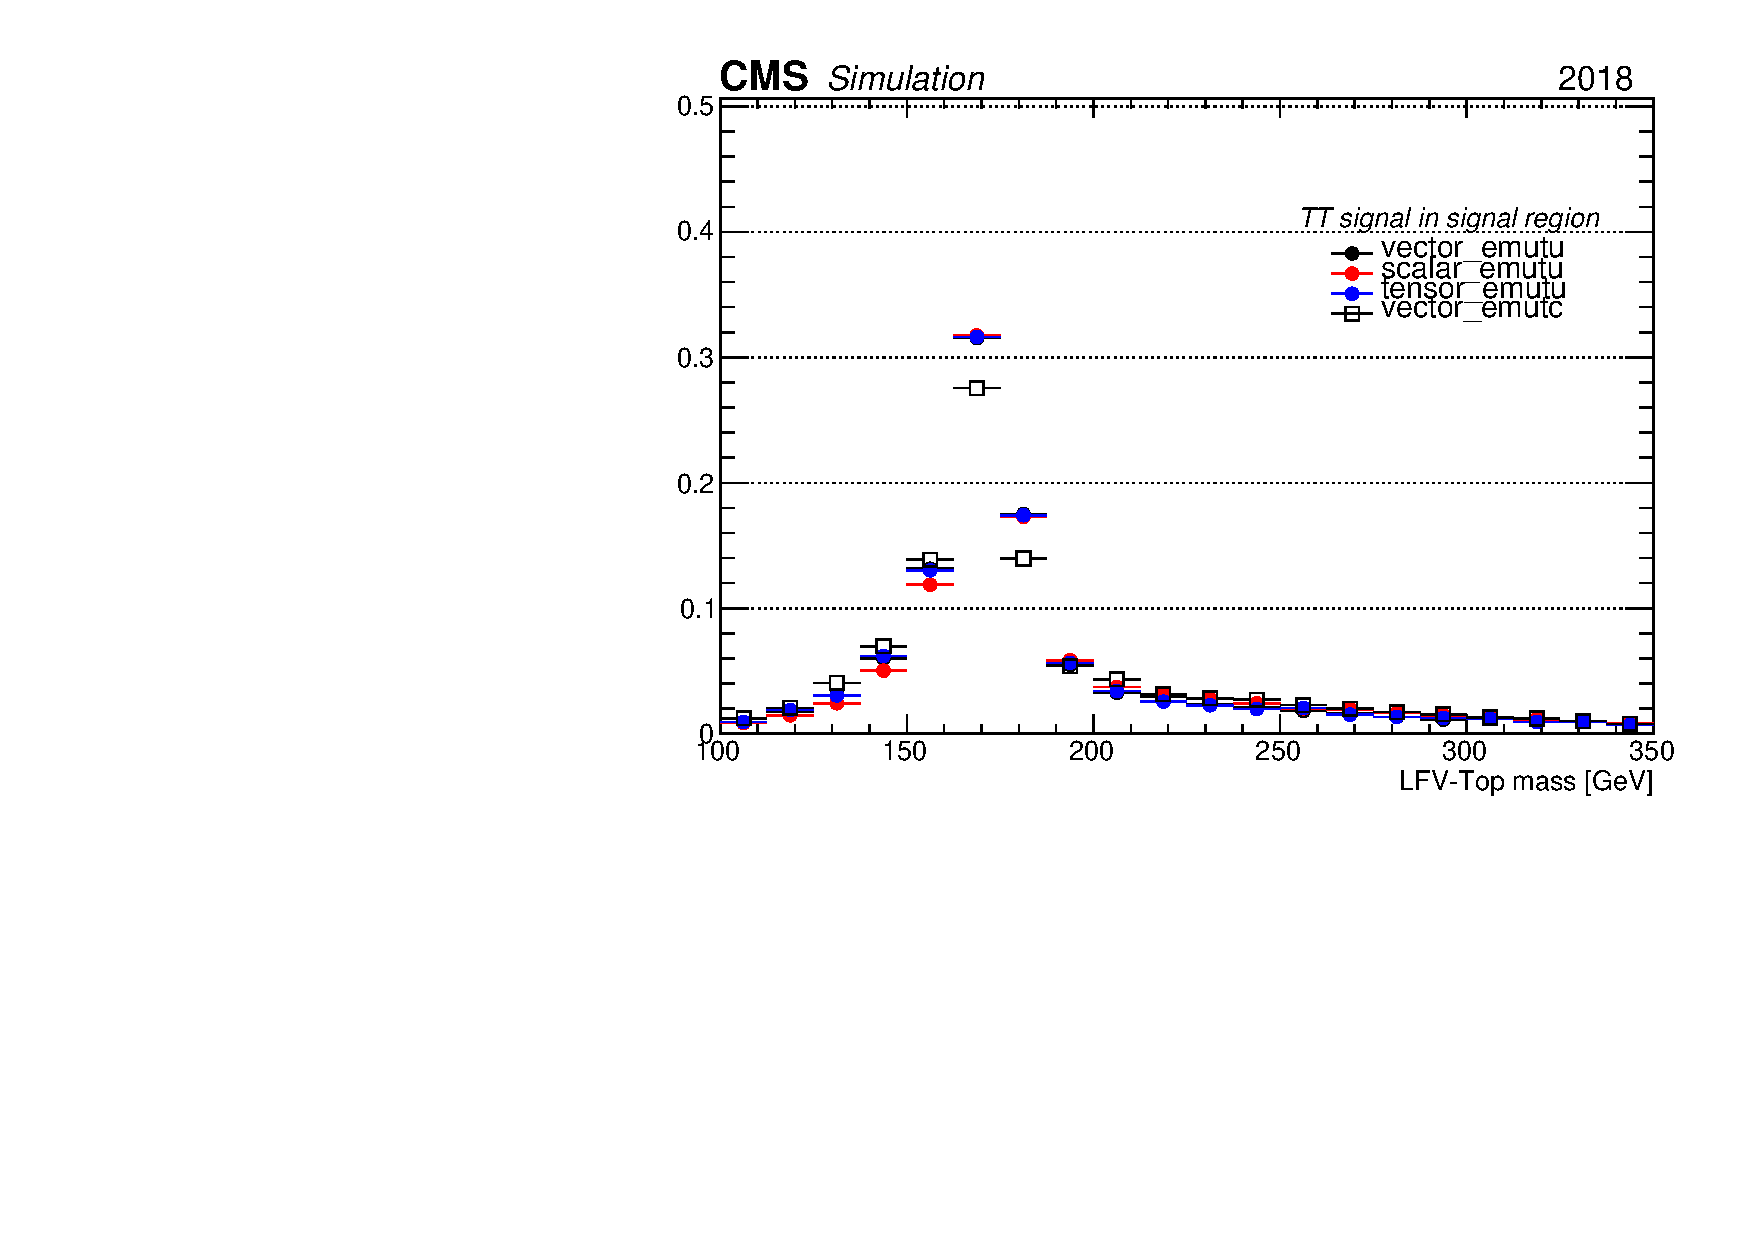
\includegraphics[width=0.48\textwidth]{figures/Part3/BDT/LFV_VR_emul_lllOffZMetg20Jetgeq1Bleq1_LFVTopmass_N}&
  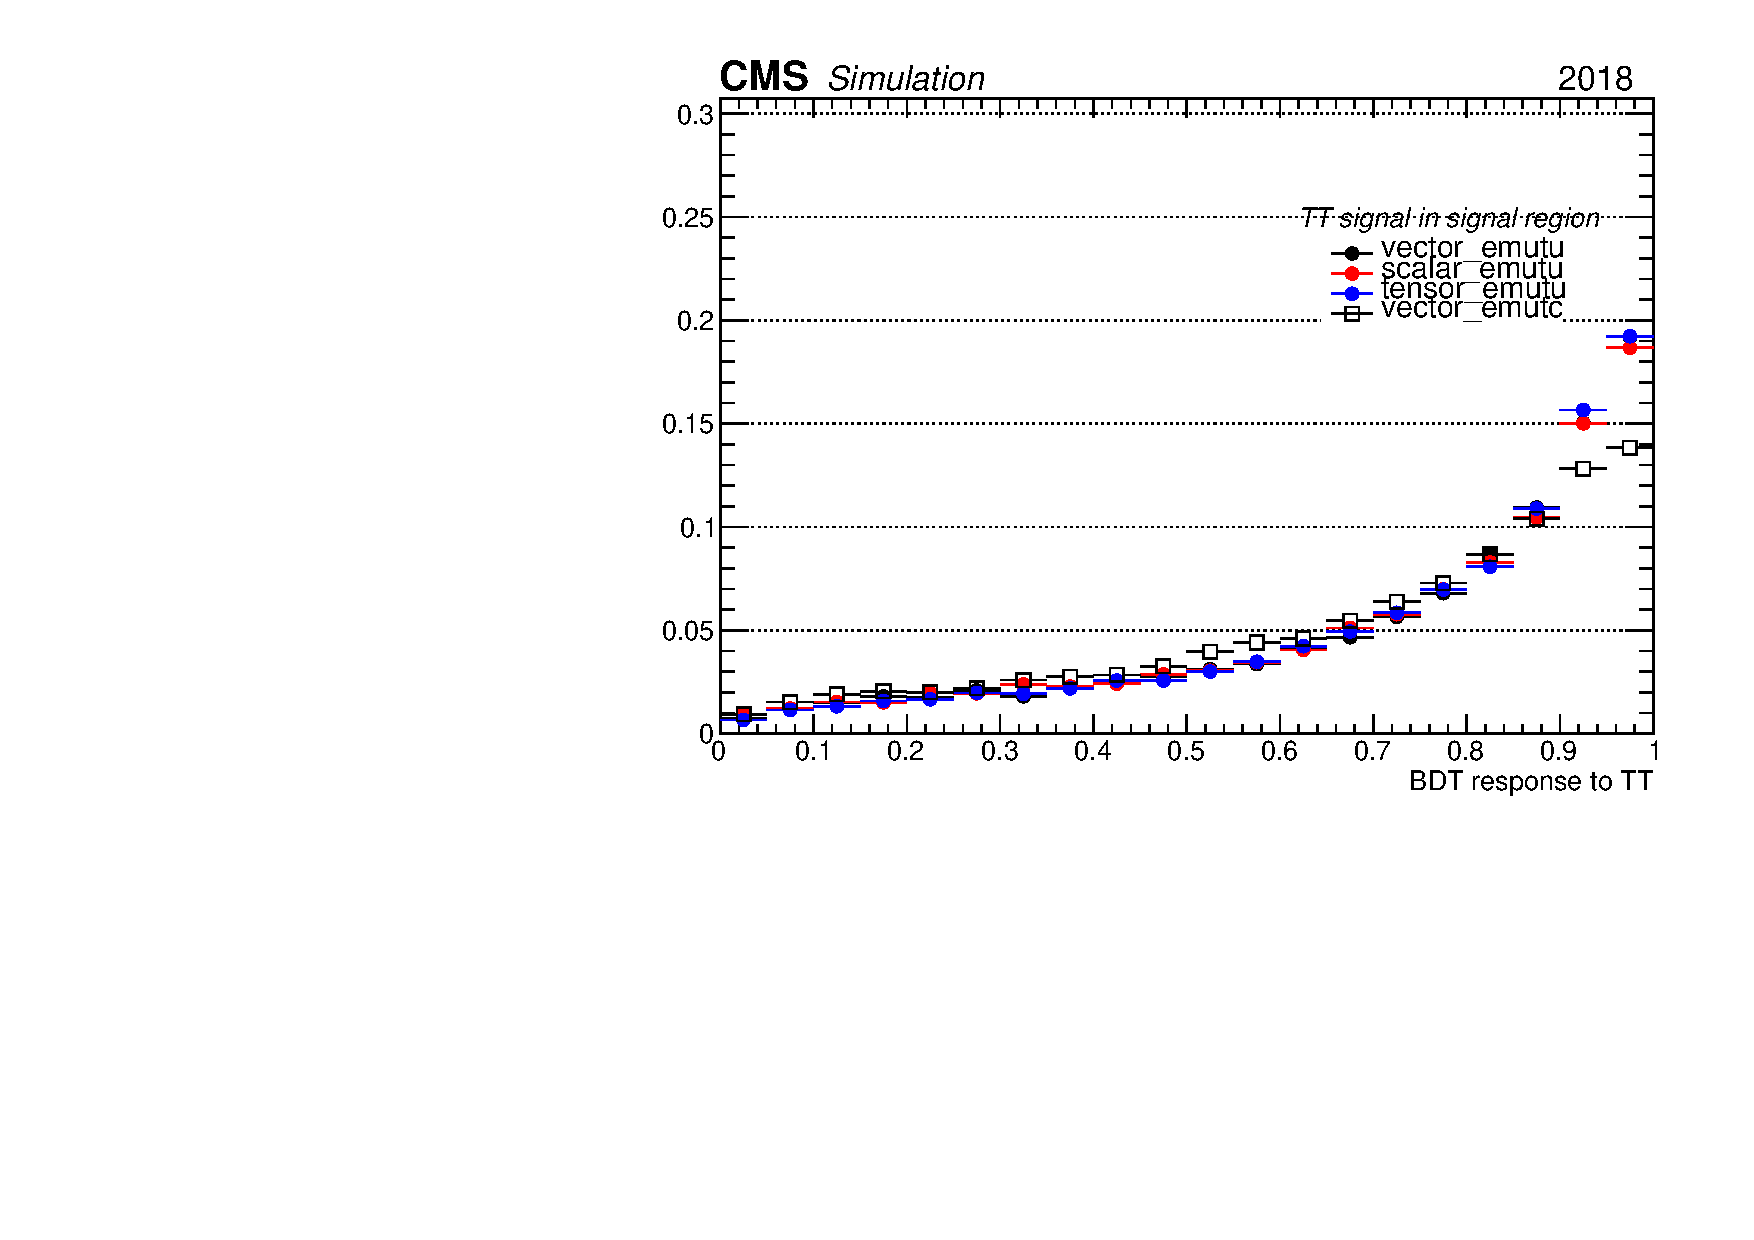
\includegraphics[width=0.48\textwidth]{figures/Part3/BDT/LFV_VR_emul_lllOffZMetg20Jetgeq1Bleq1_BDT_TT_N}\\
 \end{tabular}
 \caption{Normalized distributions of the simulated top quark decay signals in \ac{SR}1 using the 2018 dataset. From left to right: LFV top mass, BDT output. In the legend of these histograms, ``vector'', ``scalar'', and ``tensor'' denote the Lorentz structures of \ac{EFT} operators, and ``emutu(c)'' denote the $\emut{u(c)}$ interaction vertex.}
 \label{fig:Lorentz}
 \end{center}
\end{figure}

The \emph{prompt} background dataset is constructed by combining all \ac{MC} samples listed under the ``prompt'' category listed in Table~\ref{tab:MCsample}. Cross sections referenced Table~\ref{tab:MCsample} are directly used to normalize the \emph{prompt} backgrounds. The construction of the \emph{nonpeompt} background dataset is different since the \emph{nonprompt} backgrounds are modeled with the \mm, which is itself constructed from 8 \acp{AR}. Therefore, 8 \acp{AR} are constructed to collect simulated $\ttbar$ and Drell-Yan events. These events are used to form the \emph{nonprompt} dataset. Each event in the \emph{nonprompt} dataset is then ``weighted'' using the output of the \mm. Finally, the \emph{nonprompt} dataset is combined with the \emph{prompt} dataset and then divided into two datasets using a 150 GeV threshold on LFV e$\upmu$ mass. 

A technique known as the ``$k$-fold cross validation'' is used to minimize the loss of statistics when partitioning datasets into training, validation, and test sets. For each targeted \ac{SR}, the corresponding signal/background set is divided evenly into five subsets. Three out of the five subsets are used in the training while a fourth subset is used as a validation set. The fifth set is used to test the performance of the trained \ac{BDT}. A second \ac{BDT} is trained using a different combination of subsets to form training, validation, and test sets. This process is repeated five times until a unique test set no longer exists, which is illustrated in Figure~\ref{fig:5fold}. This technique ensures that the test set is always statistically independent of the process of parameters tuning, which serves as the basis for the bias-free evaluation after training: when evaluating each event using the trained model, it is always possible to pick one of the five \acp{BDT} where this particular event was not included in the training or validation.

\begin{figure}[tbh!]
 \begin{center}
  \caption{Illustration of a 5-fold cross-validation. In this setup, five \acp{BDT} are trained/tested using the same dataset arranged in different configurations. Each of the bottom five rows represents the configuration of a \ac{BDT}.}
 \begin{tabular}{c}
 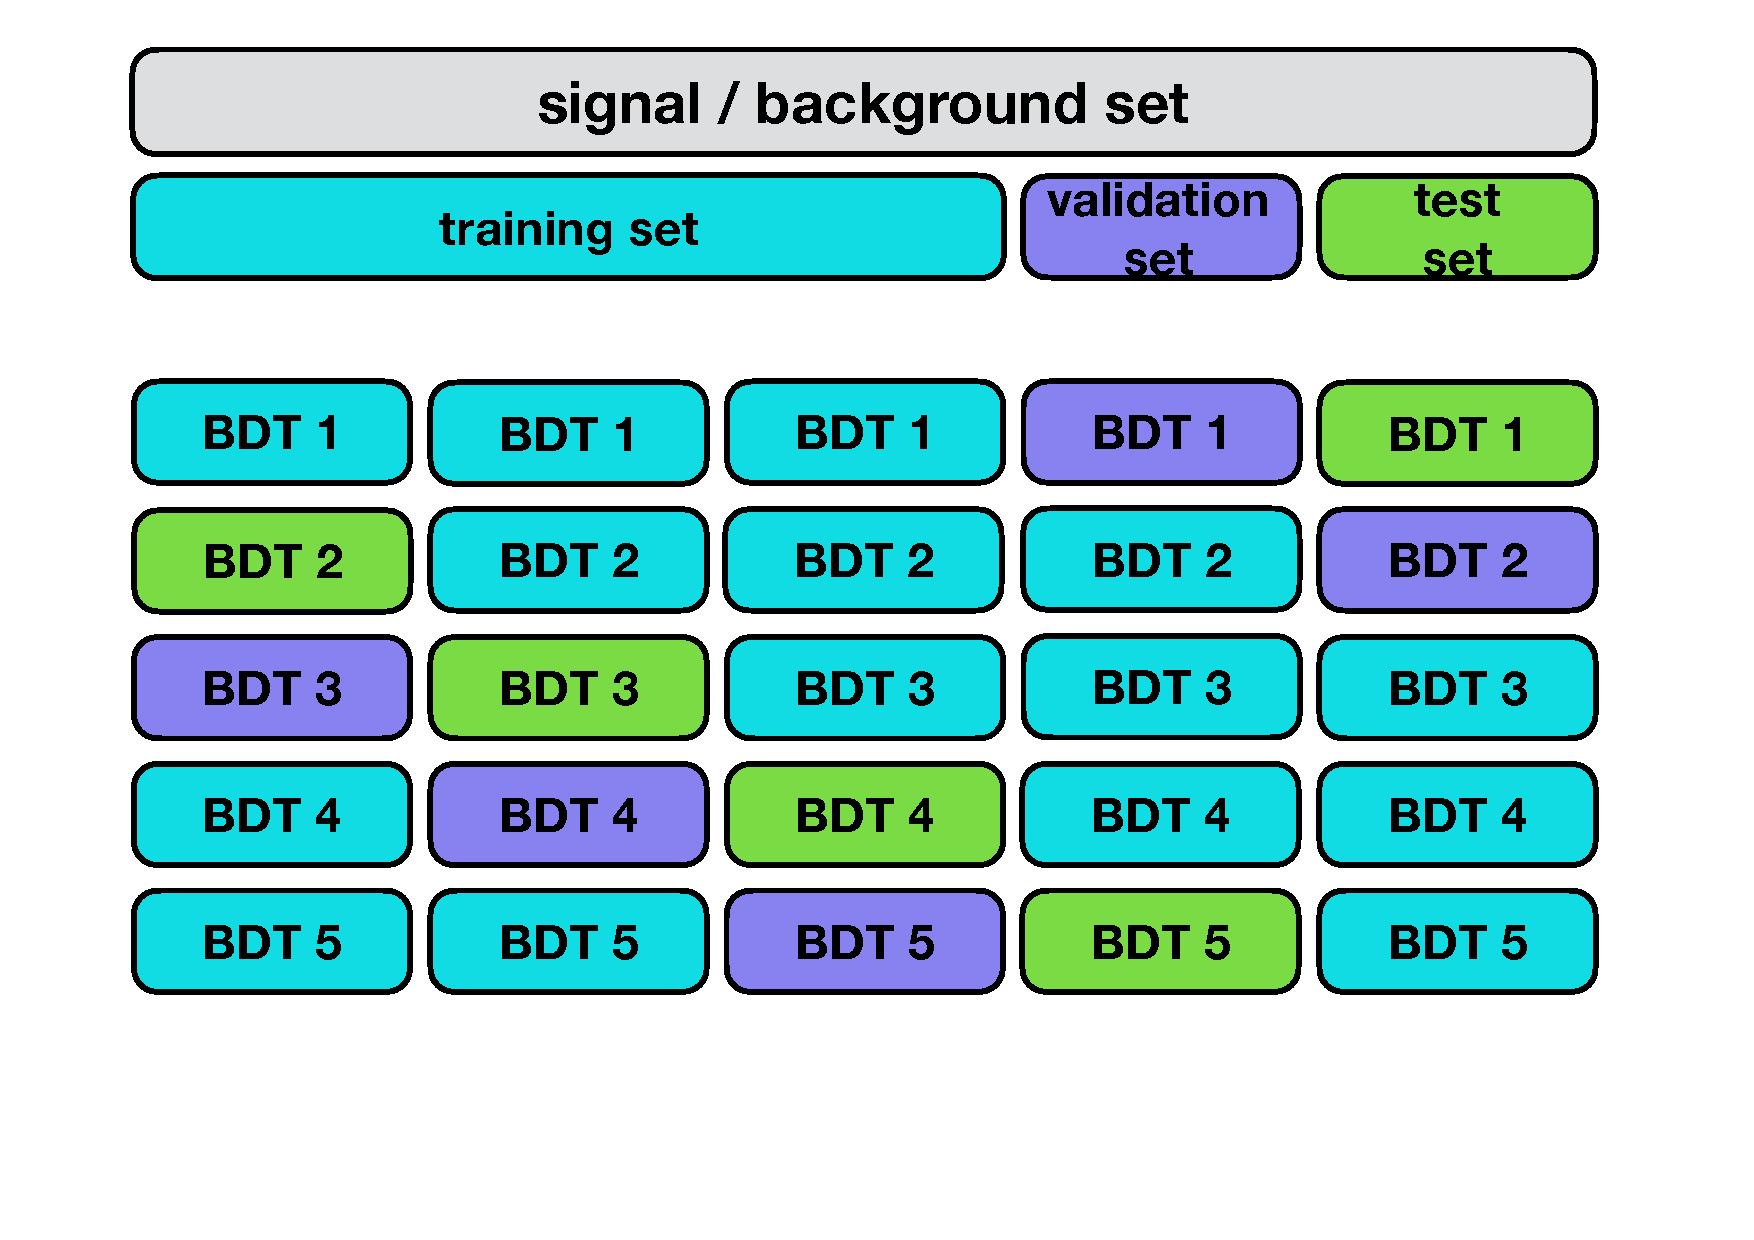
\includegraphics[width=0.8\textwidth]{figures/Part3/BDT/kfold}
 \end{tabular}
 \label{fig:5fold}
 \end{center}
\end{figure}

The same set of hyperparameters is used for all \acp{BDT}, which are optimized using a randomized grid search algorithm. The number of estimators is set to 1000 with a max depth of 5. The standard loss function implemented in \cite{Chen:2016:XST:2939672.2939785} is used as the evaluation metric. The performance of the \ac{BDT} is visualized using a metric known as ``\ac{ROC} curve'', which is shown in Figure \ref{fig:ROC}. In general, the \acp{BDT} trained in \ac{SR}2 (i.e. $\textsf{m}(\textsf{e}\upmu)~>$ 150 GeV) are much more performant due to the high $\pt$ objects in the final states.

\begin{figure}[tbh!]
 \begin{center}
 \begin{tabular}{cc}
 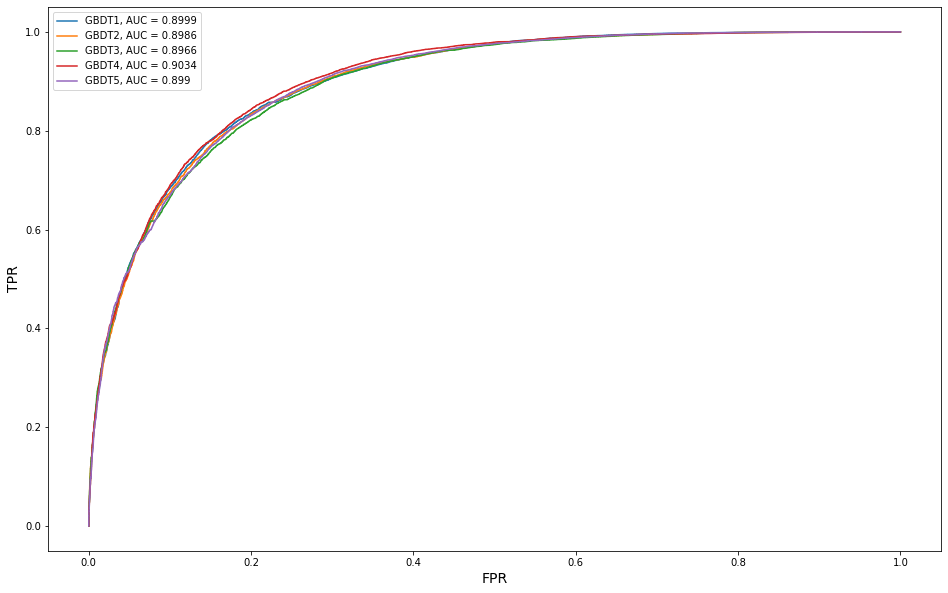
\includegraphics[width=0.48\textwidth]{figures/Part3/BDT/5foldTT}&
  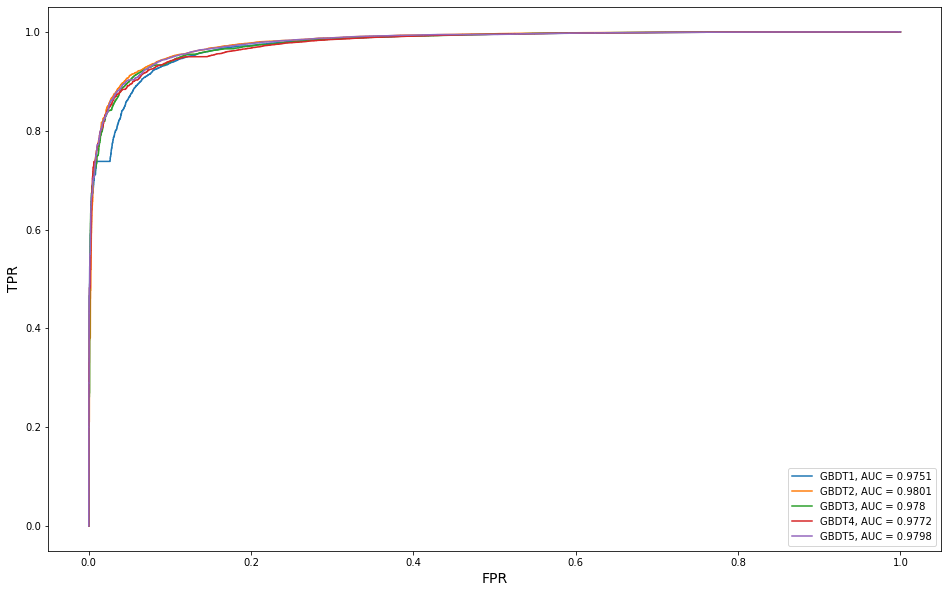
\includegraphics[width=0.48\textwidth]{figures/Part3/BDT/5foldST}\\
 \end{tabular}
 \caption{\ac{ROC} curves extracted using the test sets specified in the 5-fold cross-validation. The left (right) figure shows the \ac{ROC} curves of the \acp{BDT} trained in \ac{SR}1 (\ac{SR}2). The area under the \ac{ROC} curves are showed in the legends.}
 \label{fig:ROC}
 \end{center}
\end{figure}
%%%%%%%%%%%%%%%%%%%%%%%%%%%%%%%%%%%%%%%%%%%%%%%%%%%%%%%%
%%%%%%%%%%%%%%%%%%%%%%%%%%%%%%%%%%%%%%%%%%%%%%%%%%%%%%%%

\section{BDT Features}
\label{sec:Input}

The discriminating variables used as input in training are referred to as "features" in this analysis. A total of 14 features are used for \ac{BDT} trained in \ac{SR}1 and \ac{SR}2. The names and descriptions of these 14 features are summarized in Table~\ref{tab:CommonFeatures}. Many of these features are derived from reconstructed heavy objects which are described in \autoref{sec:Kin}.


\begin{table}[th]
\sffamily
\centering
\caption{Features shared by \ac{BDT}s trained in both \ac{SR}1 and \ac{SR}2.}
 \resizebox{\linewidth}{!}{%
\begin{tabular}{lc}
\toprule
Name & Description \\
\midrule
MVA\_Memu & invariant mass of the LFV-e$\upmu$ pair\\
MVA\_LFVePt & $\pt$ of the LFV electron \\
MVA\_LFVmuPt & $\pt$ of the LFV muon \\
MVA\_LFVTopmass & invariant mass of the LFV top quark candidate \\
MVA\_Zmass & invariant mass of Z boson candidate \\
MVA\_Jet2Btag & b-tagging score of the jet with the second highest b-tagging score \\
MVA\_Mbl2 & invariant mass of the second $\mbl$ system \\
MVA\_njet & number of jets \\
MVA\_nbjet & number of b-tagged jets \\
MVA\_tM & transverse mass of the W boson candidate (from the \ac{SM} top quark) \\
MVA\_llDr & $\mathrm{\Delta}R$ between LFV electron and LFV muon \\
MVA\_SSee\_Zmass & invariant mass of a Same-Sign di-electron pair \\
MVA\_Topmass & invariant mass of the \ac{SM} top quark candidate \\
MVA\_Met & missing transverse momentum (\ac{MET}) \\
\bottomrule
\end{tabular}
}
\label{tab:CommonFeatures}
\end{table}

Four additional features are added to the \ac{BDT} trained in \ac{SR}1. The ``MVA\_JeDr'' and ``MVA\_JeDr'' variables are defined by using the jet that forms the LFV top quark candidate and calculating the opening angle between this jet and the LFV leptons. It is expected that this angle is smaller in the LFV decay mode than LFV production mode. Two additional features are added to the \ac{BDT} trained in SR2. A description of how the standalone lepton is determined can be found in \autoref{sec:Kin}. 

\begin{table}[th]
\sffamily
\centering
\caption{Features only used by \ac{BDT} trained in \ac{SR}1}
 \resizebox{0.8\linewidth}{!}{%
\begin{tabular}{lc}
\toprule
Name & Description \\
\midrule
MVA\_Ht & scalar sum of the $\pt$ of all jets and leptons \\
MVA\_Mbl1 & invariant mass of the second $\mbl$ system \\
MVA\_JeDr & $\mathrm{\Delta}R$ between LFV electron and a light jet (non b jet) \\
MVA\_JmuDr & $\mathrm{\Delta}R$ between LFV muon and a light jet (non b jet) \\
\bottomrule
\end{tabular}
}
\label{tab:SR1Features}
\end{table}

\begin{table}[th]
\sffamily
\centering
\caption{Features only used by \ac{BDT} trained in \ac{SR}2}
 \resizebox{0.52\linewidth}{!}{%
\begin{tabular}{lc}
\toprule
Name & Description \\
\midrule
MVA\_BaPt & $\pt$ of the standalone lepton \\
MVA\_JetHt & scalar sum of the $\pt$ of all jets \\
\bottomrule
\end{tabular}
}
\label{tab:SR2Features}
\end{table}

Distributions of selected features are shown in Figure \ref{fig:Features1}-\ref{fig:Features5}. Distributions of the full list of features can be found in \autoref{chap:SRMC}. The relative importance of these features is extracted using the "gain" method and is shown in Figure \ref{fig:Ranking}. The correlations between different features are shown in Figure~\ref{fig:Corr1}-\ref{fig:Corr2}.

\begin{figure}[tbh!]
 \begin{center}
 \begin{tabular}{c}
 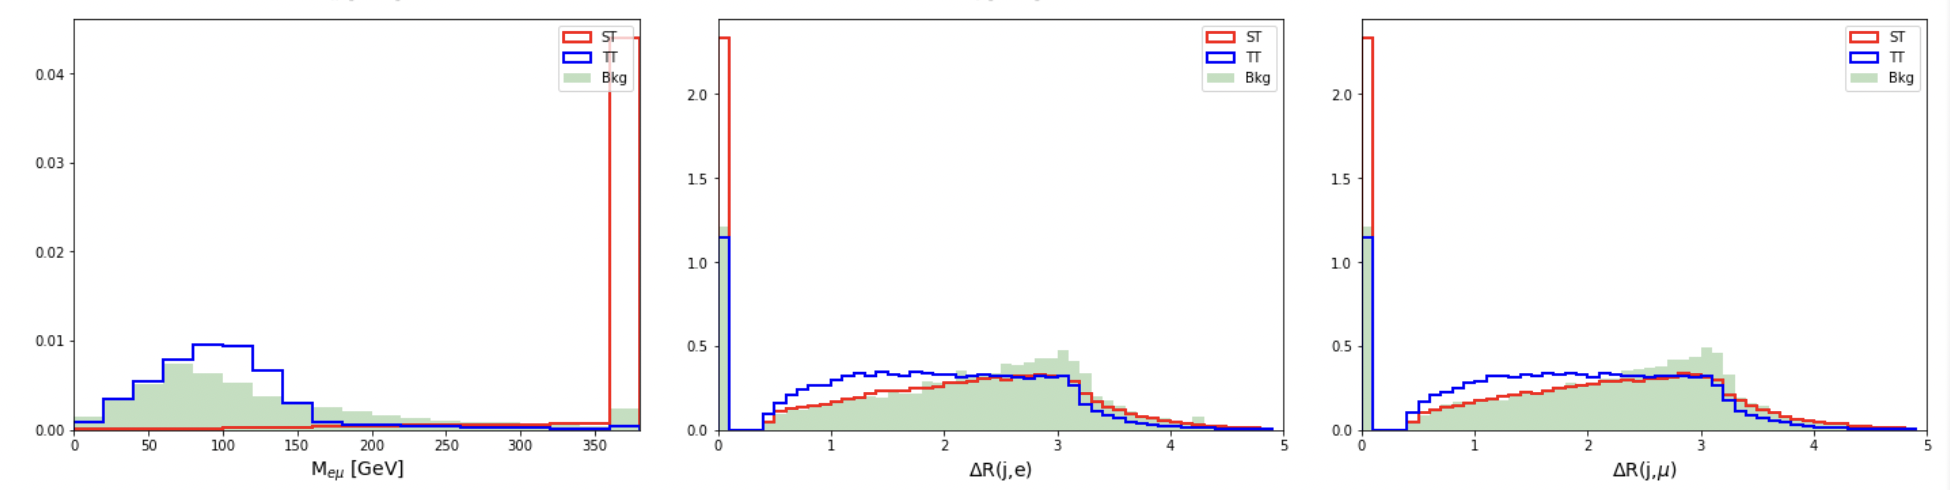
\includegraphics[width=0.99\textwidth]{figures/Part3/BDT/Features1}\\
 \end{tabular}
 \caption{Normalized distribution of various features in SR. From left to right: MVA\_M$_{e\mu}$, MVA\_JeDr, MVA\_JeDr.}
 \label{fig:Features1}
 \end{center}
\end{figure}

\begin{figure}[tbh!]
 \begin{center}
 \begin{tabular}{c}
 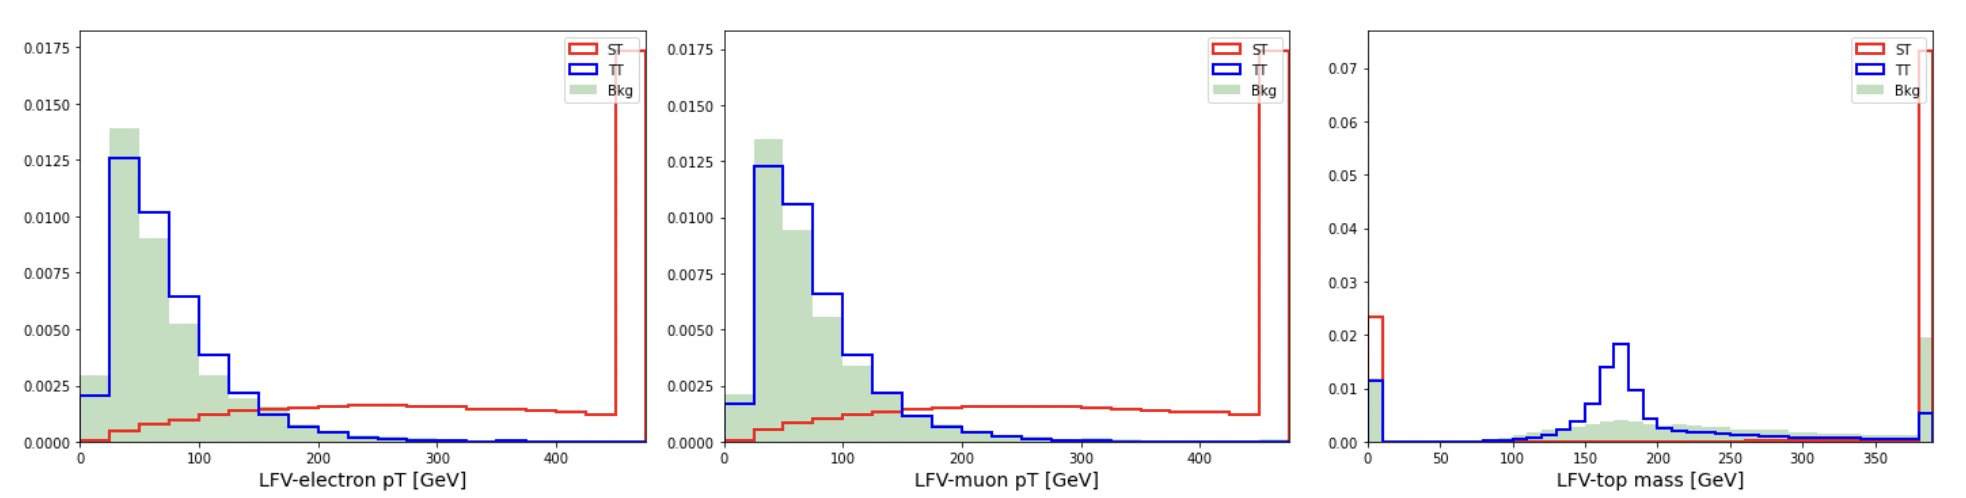
\includegraphics[width=0.99\textwidth]{figures/Part3/BDT/Features2}\\
 \end{tabular}
 \caption{Normalized distribution of additional features in SR. From to left to right: MVA\_LFVePt, MVA\_LFVmuPt, MVA\_LFVTopmass.}
 \label{fig:Features2}
 \end{center}
\end{figure}

\begin{figure}[tbh!]
 \begin{center}
 \begin{tabular}{c}
 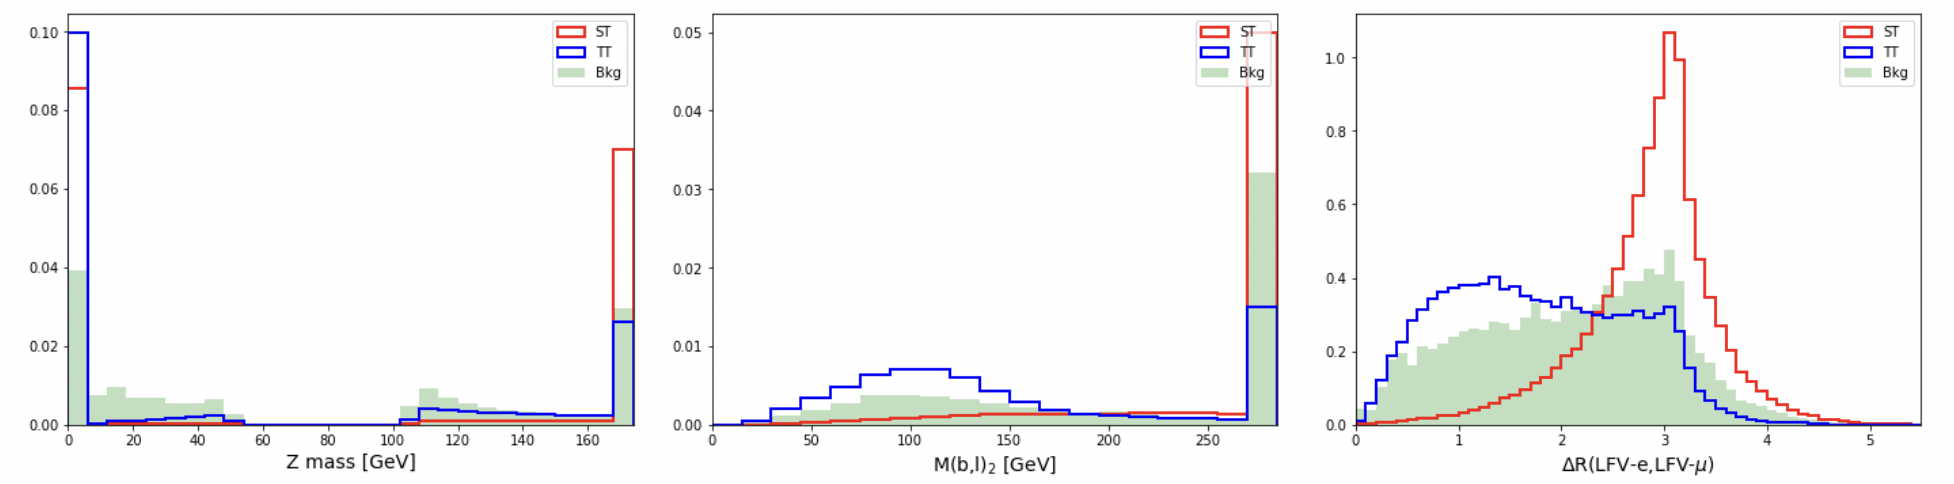
\includegraphics[width=0.99\textwidth]{figures/Part3/BDT/Features3}\\
 \end{tabular}
 \caption{Normalized distribution of additional features in SR. From left to right: MVA\_Zmass, MVA\_Mbl2, MVA\_llDr.}
 \label{fig:Features3}
 \end{center}
\end{figure}

\begin{figure}[tbh!]
 \begin{center}
 \begin{tabular}{c}
 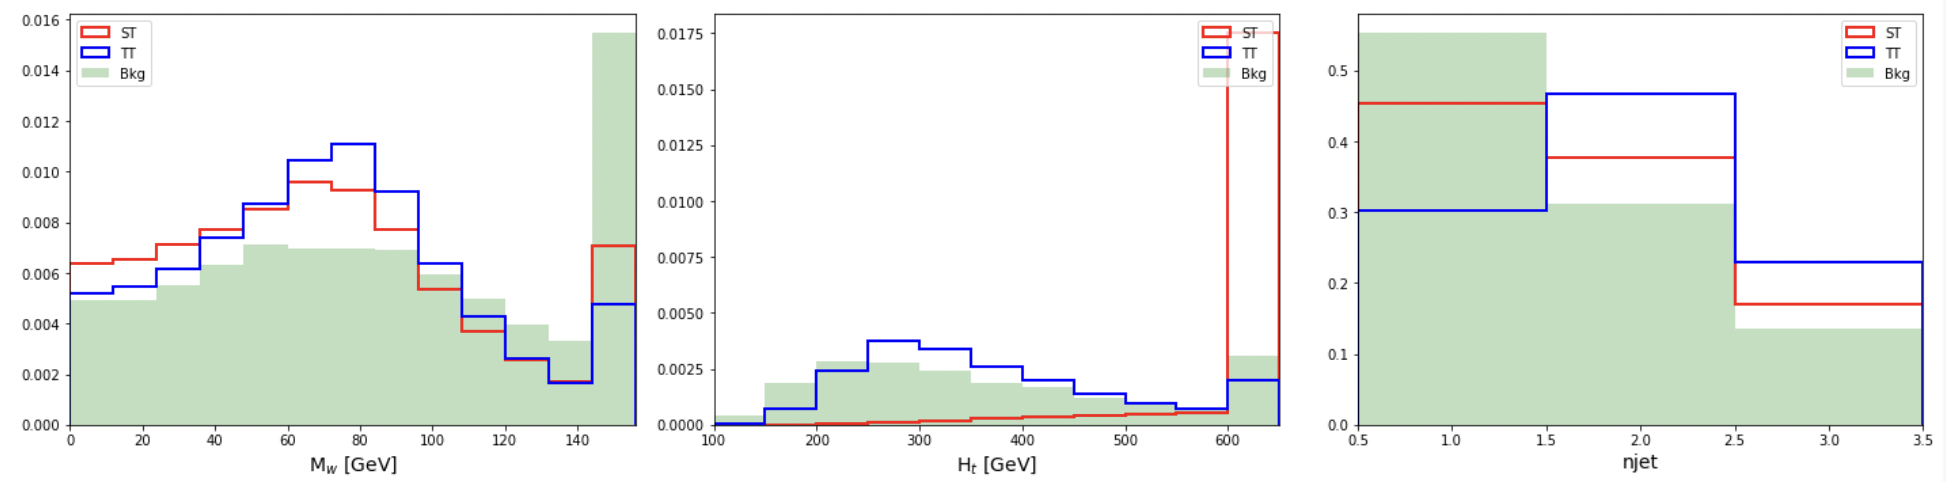
\includegraphics[width=0.99\textwidth]{figures/Part3/BDT/Features4}\\
 \end{tabular}
 \caption{Normalized distribution of additional features in SR. From left to right: MVA\_tM, MVA\_Ht, MVA\_njet.}
 \label{fig:Features4}
 \end{center}
\end{figure}

\begin{figure}[tbh!]
 \begin{center}
 \begin{tabular}{c}
 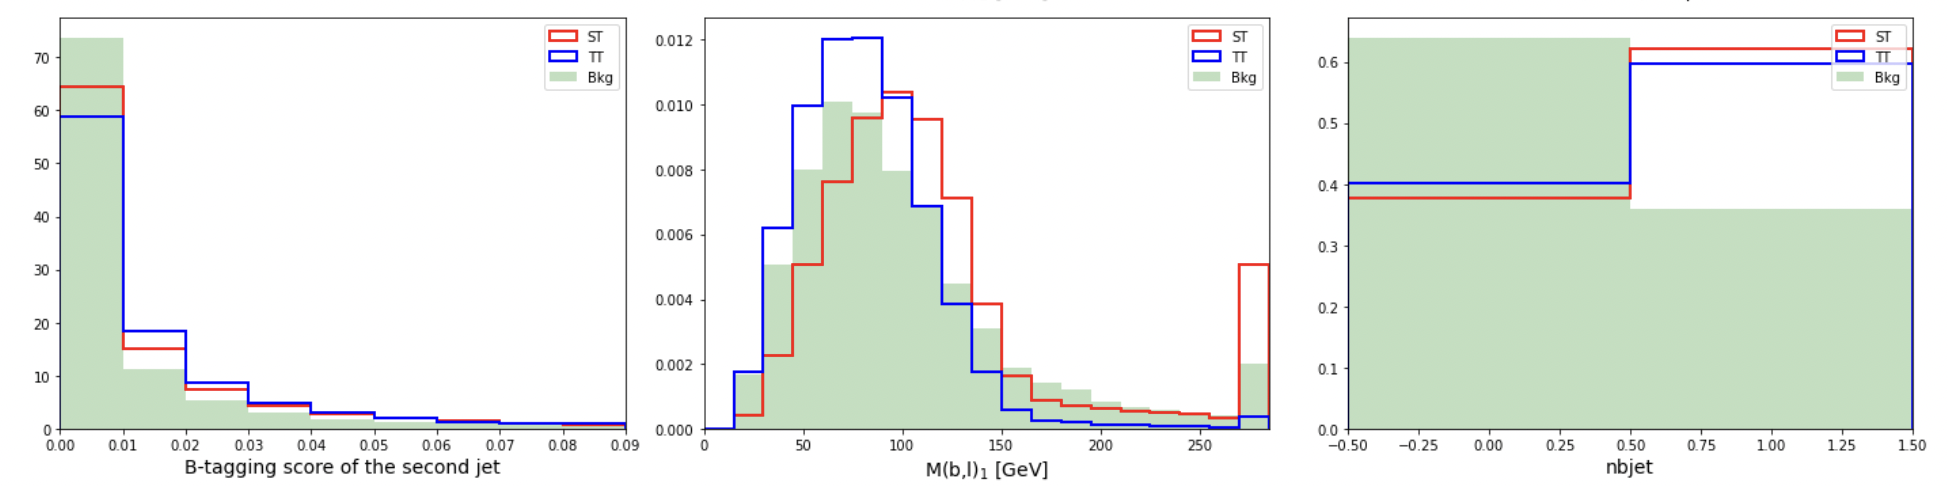
\includegraphics[width=0.99\textwidth]{figures/Part3/BDT/Features5}\\
 \end{tabular}
 \caption{Normalized distribution of additional features in SR. From left to right: MVA\_Jet2Btag, MVA\_Mbl1, MVA\_nbjet.}
 \label{fig:Features5}
 \end{center}
\end{figure}

\begin{figure}[tbh!]
 \begin{center}
 \begin{tabular}{cc}
 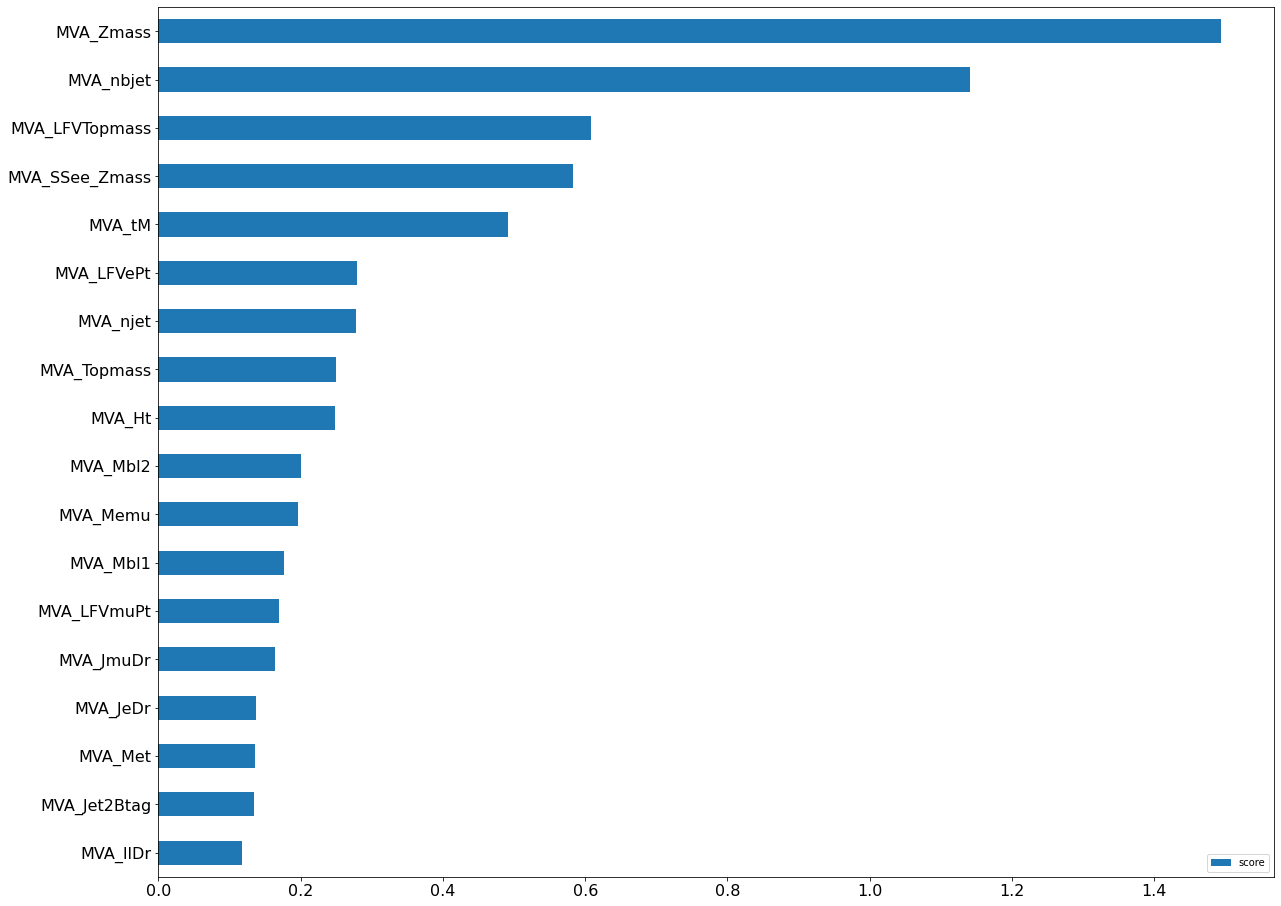
\includegraphics[width=0.48\textwidth]{figures/Part3/BDT/TTranking}&
 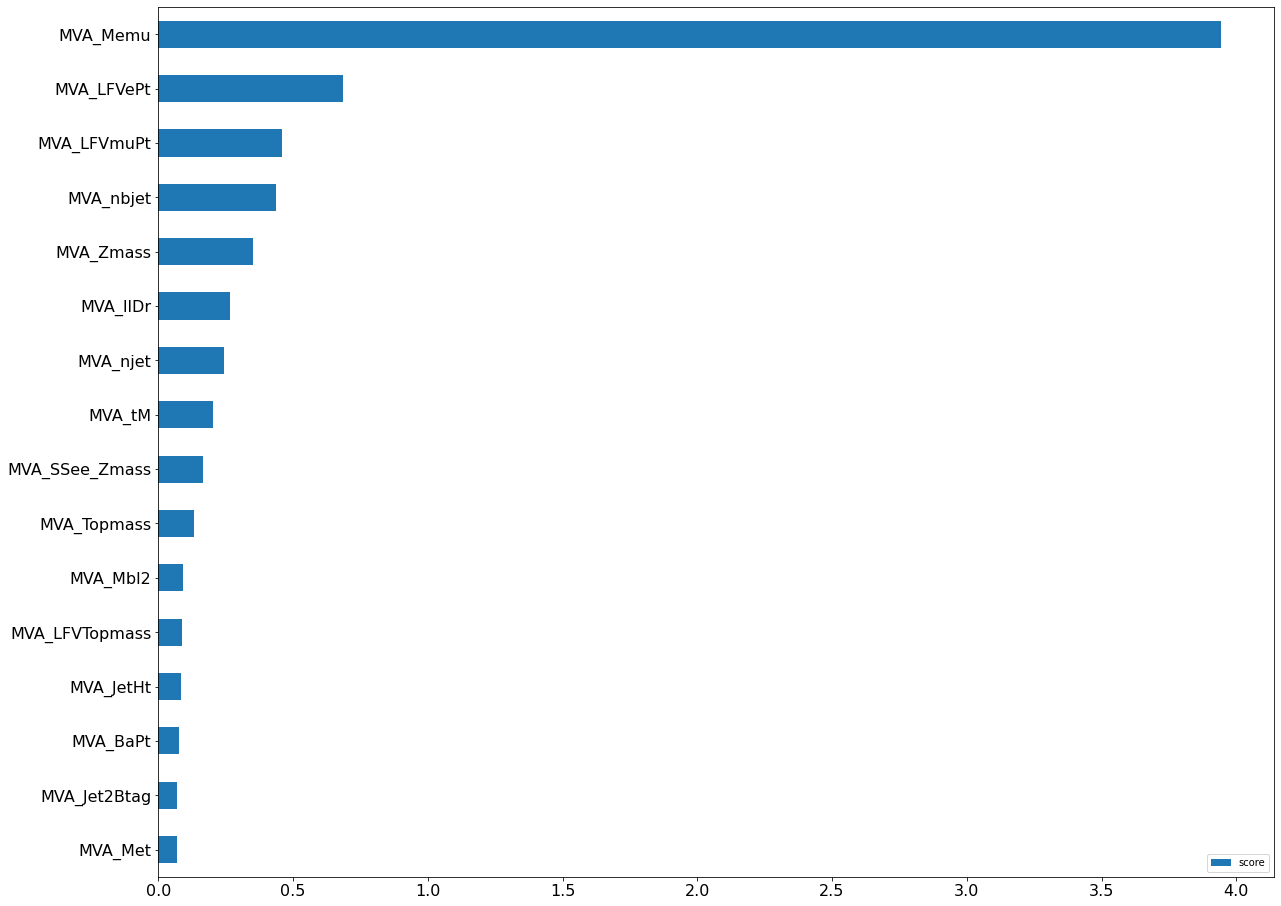
\includegraphics[width=0.48\textwidth]{figures/Part3/BDT/STranking}\\
 \end{tabular}
 \caption{List of features ranked by their relative importance. From left to right: BDT targeting TT (SR1), BDT targeting ST (SR2)}
 \label{fig:Ranking}
 \end{center}
\end{figure}

\begin{figure}[tbh!]
 \begin{center}
 \begin{tabular}{cc}
 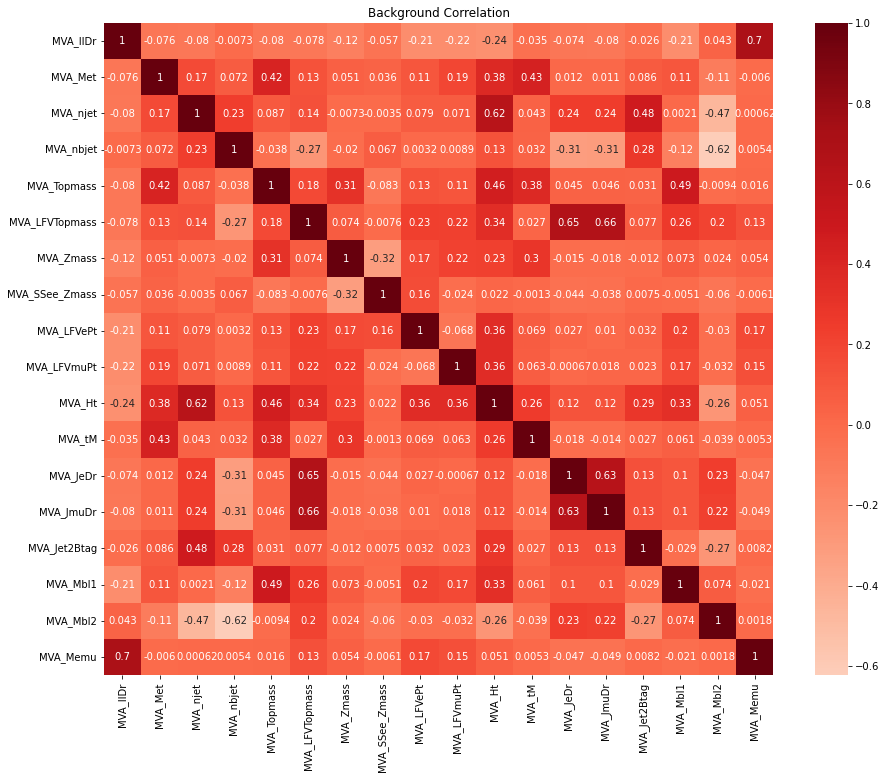
\includegraphics[width=0.48\textwidth]{figures/Part3/BDT/corr_bkg_SR1}&
 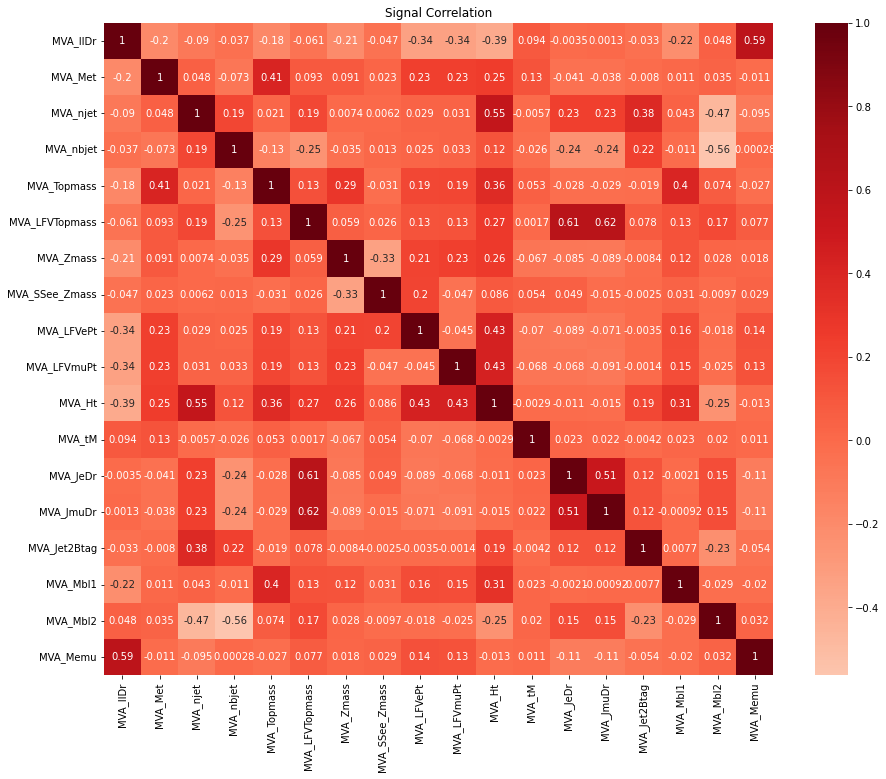
\includegraphics[width=0.48\textwidth]{figures/Part3/BDT/corr_signal_SR1}\\
 \end{tabular}
 \caption{Correlation matrices (SR1), from left to right: background correlation, signal correlation.}
 \label{fig:Corr1}
 \end{center}
\end{figure}

\begin{figure}[tbh!]
 \begin{center}
 \begin{tabular}{cc}
 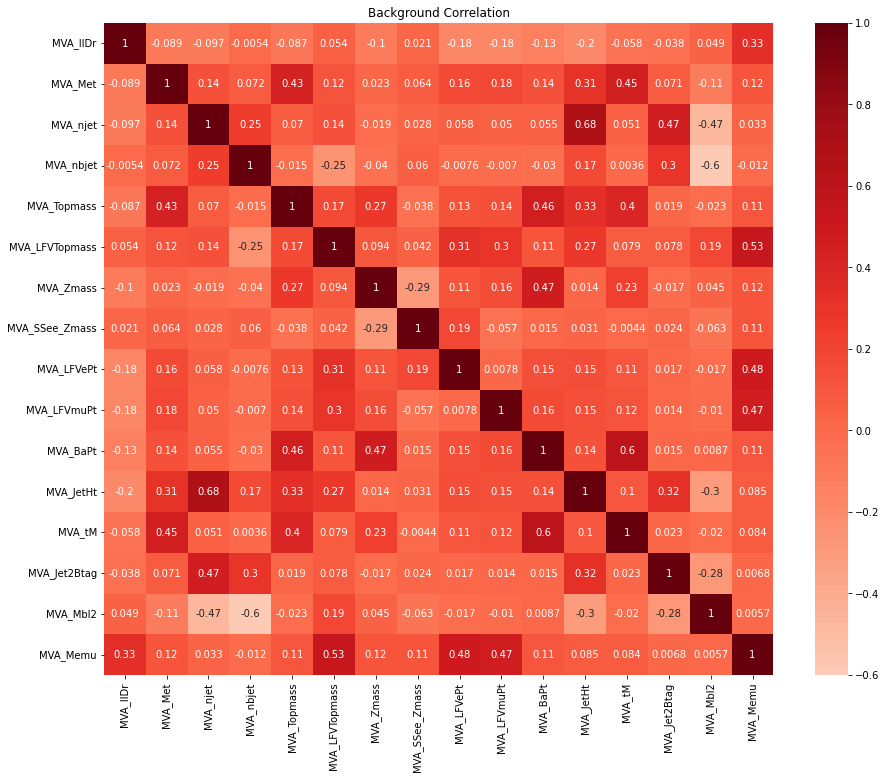
\includegraphics[width=0.48\textwidth]{figures/Part3/BDT/corr_bkg_SR2}&
 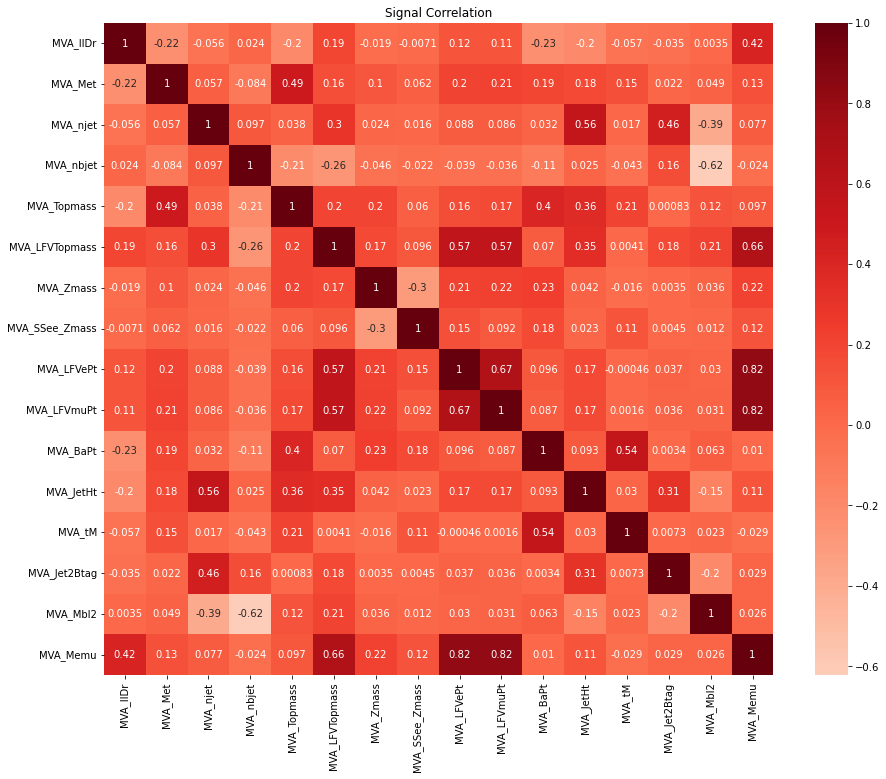
\includegraphics[width=0.48\textwidth]{figures/Part3/BDT/corr_signal_SR2}\\
 \end{tabular}
 \caption{Correlation matrices (SR2), from left to right: background correlation, signal correlation.}
 \label{fig:Corr2}
 \end{center}
\end{figure}
%%%%%%%%%%%%%%%%%%%%%%%%%%%%%%%%%%%%%%%%%%%%%%%%%%%%%%%%
%%%%%%%%%%%%%%%%%%%%%%%%%%%%%%%%%%%%%%%%%%%%%%%%%%%%%%%%

\section{BDT Output}
\label{sec:Output}

The output of the \acp{BDT} in \acp{SR} are shown in Figure \ref{fig:bdt_output}. The \emph{nonprompt} background is estimated with the matrix method. Other backgrounds are estimated with \ac{MC} simulation.

\begin{figure}[tbh!]
 \begin{center}
 \begin{tabular}{cc}
 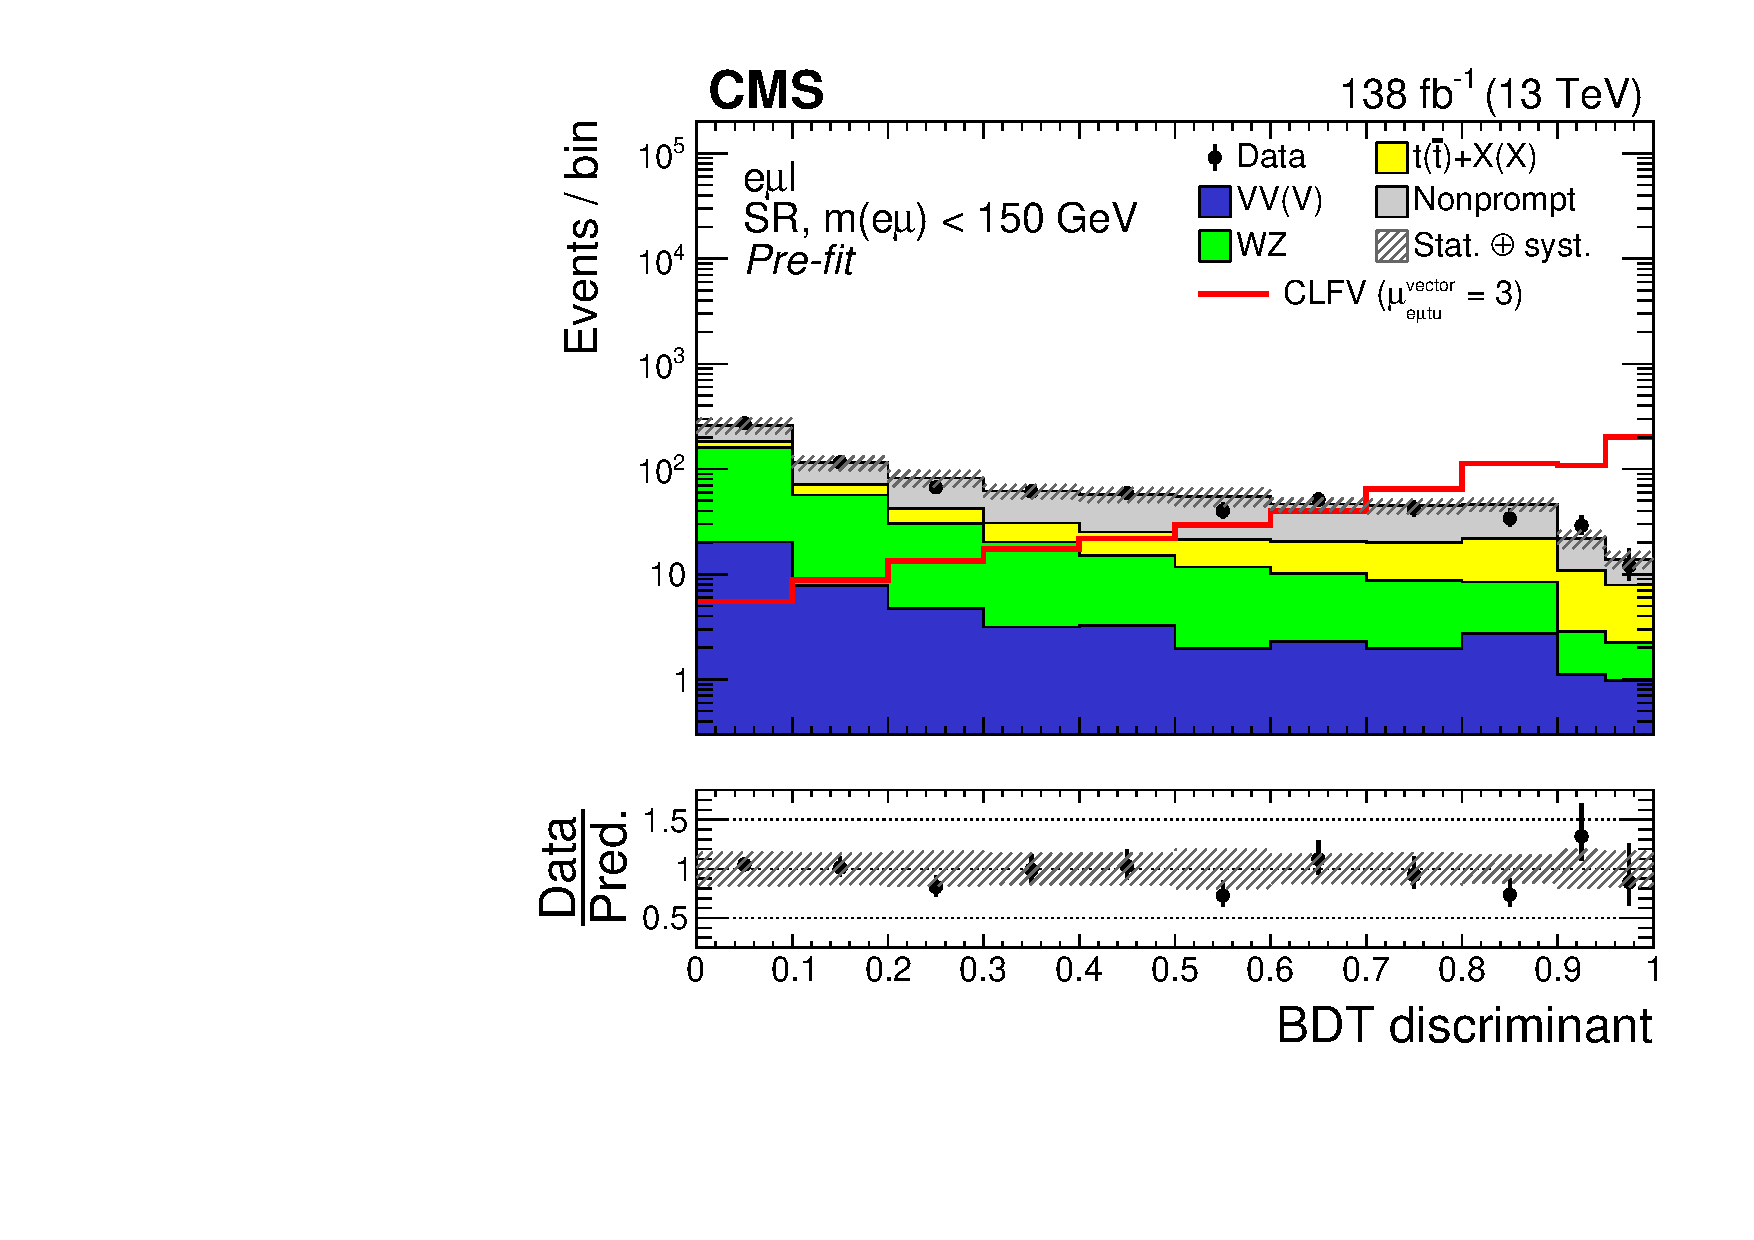
\includegraphics[width=0.48\textwidth]{figures/Part3/BDT/BDT_TT}&
 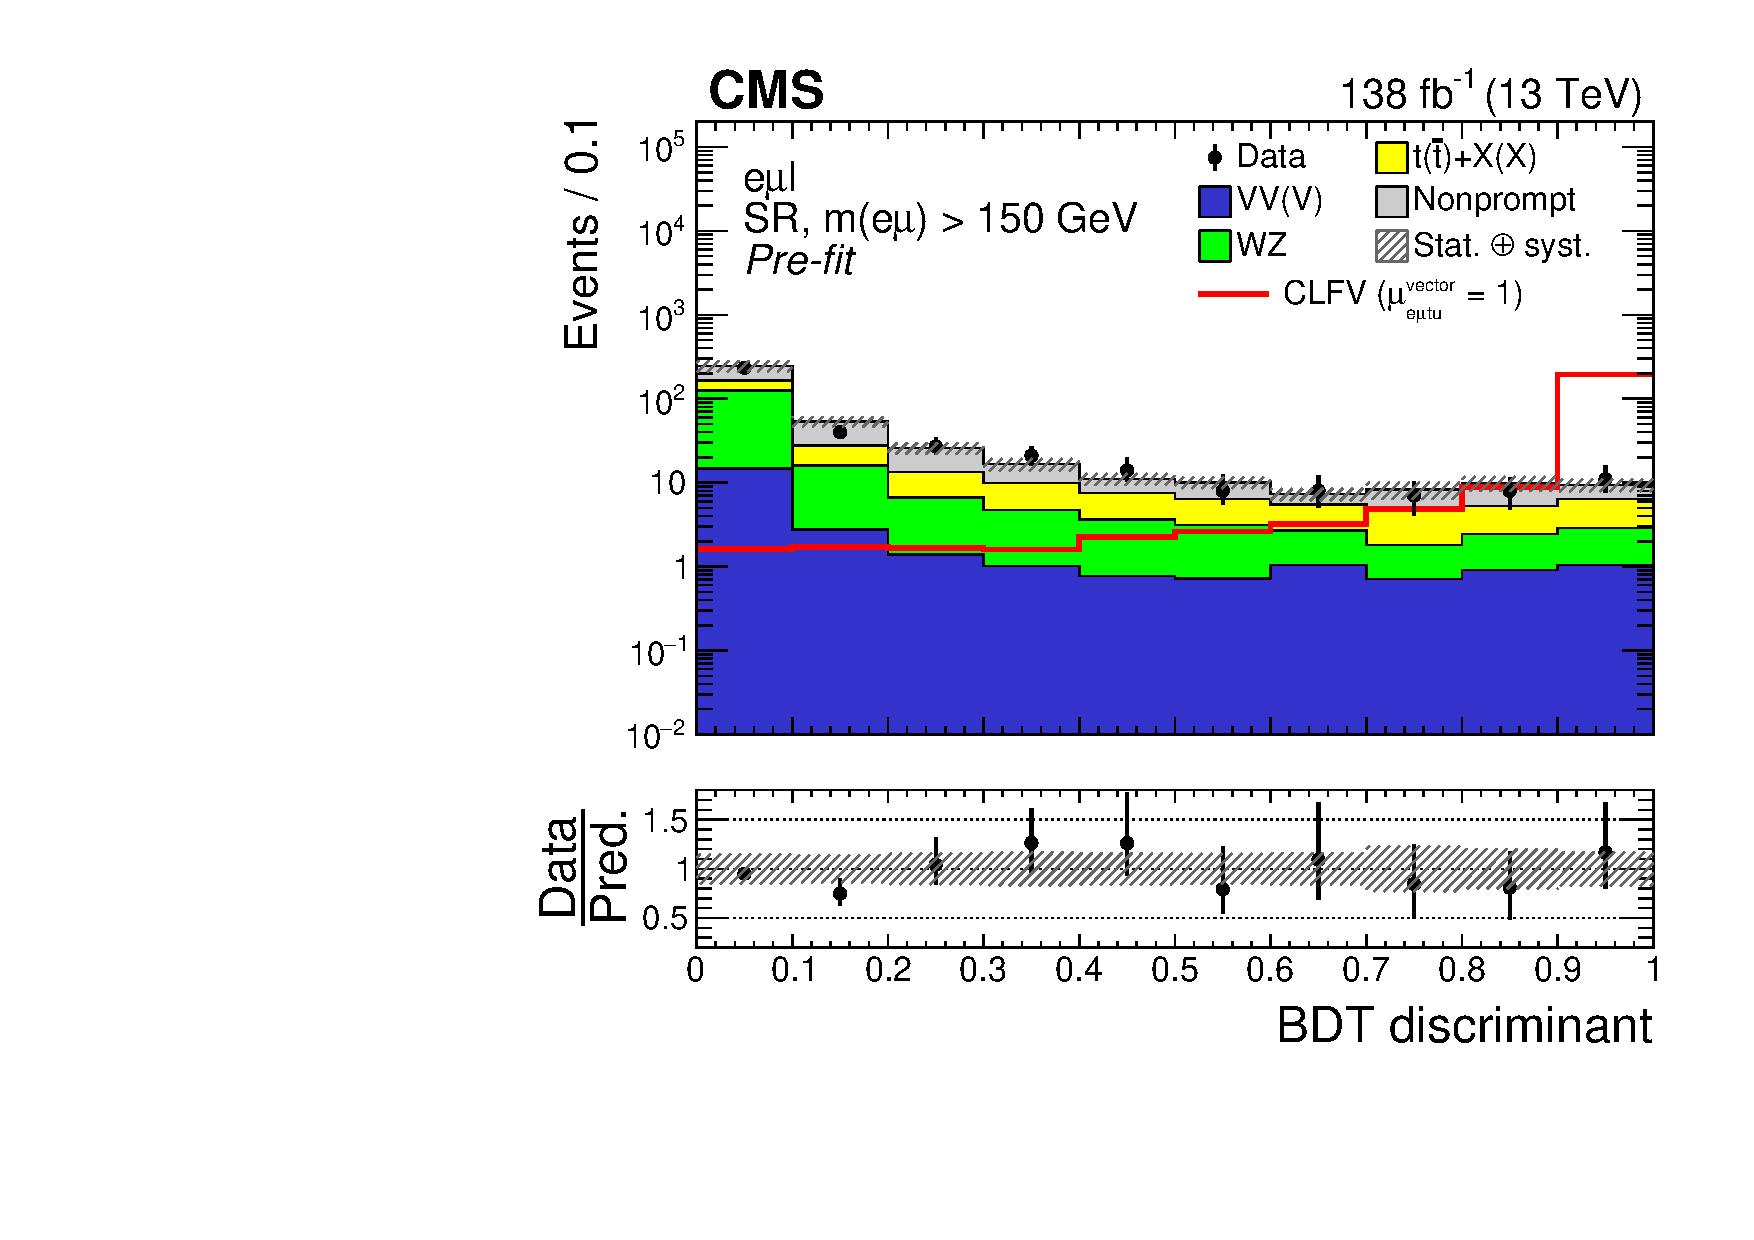
\includegraphics[width=0.48\textwidth]{figures/Part3/BDT/BDT_ST}\\
 \end{tabular}
 \caption{Distributions of the \ac{BDT} discriminator targeting the \ac{CLFV} top quark decay (left) and production (right) signal. Contributions from the two signal modes (production and decay) are combined within each \ac{SR} and are shown as the solid red line. The pre-fit signal strength ($\mu_{\emut{u}}^{\textsf{vector}}$ = 1), corresponding to $\textsf{C}_{\emut{u}}^{\textsf{vector}}/\Lam^2~=~1~\TeV^{\textsf{-2}}$, is used to normalise the signal cross sections. The hatched bands indicate statistical and systematic uncertainties for the background predictions.}
 \label{fig:bdt_output}
 \end{center}
\end{figure}